\documentclass{beamer}
\usepackage[spanish]{babel}
\usepackage[utf8]{inputenc}
\usepackage{graphicx}
\graphicspath{ {./images/}}

\usetheme{Madrid}
\usecolortheme{default}

%------------------------------------------------------------
%This block of code defines the information to appear in the
%Title page
\title[PC1 Estadistica Aplicada] %optional
{Aplicacion de tecnicas de estimacion y prueba de hipotesis}

\subtitle{
  Caso: tendencias socio-economicas de algunas
  lineas de carrea de Ingenieria de sistemas
}

\author % (optional)
{
  Alvarez \and Bautista \and Burga \and
  Casanova \and  Cuyate
}

\institute
{
  Facultad de Ingenieria Industrial y de Sistemas\\
  \textbf{Universidad Nacional de Ingenieria}
}

\date
{Octubre 2022}

% \logo{\includegraphics[height=1cm]{overleaf-logo}}

%End of title page configuration block
%------------------------------------------------------------

%------------------------------------------------------------
%The next block of commands puts the table of contents at the
%beginning of each section and highlights the current section:

\AtBeginSection[]
{
  \begin{frame}
    \frametitle{Tabla de Contenido}
    \tableofcontents[currentsection]
  \end{frame}
}
%------------------------------------------------------------


\begin{document}

%The next statement creates the title page.
\frame{\titlepage}


%---------------------------------------------------------
%This block of code is for the table of contents after
%the title page
\begin{frame}
\frametitle{Tabla de Contenido}
\tableofcontents
\end{frame}
%---------------------------------------------------------

\section{Problema}

\begin{frame}
\frametitle{Problematica}

\begin{itemize}
    \item Empiricamente se observa que en el mundo la precarizacion del trabajo
se acrecenta cada vez mas, de igual modo con la evolucion
    de personas casadas y los salarios promedio de los jovenes
    \item Con motivo de generar informacion util para la prediccion de estas tendencias
socio-economicas se ha procedio a realizar un analisis estadistico sobre
9 hipotesis planteadas

\end{itemize}
\end{frame}



%---------------------------------------------------------
\section{Objetivos}

%---------------------------------------------------------
\begin{frame}

\frametitle{Objetivos del trabajo}

\begin{alertblock}{General}
  Generar informacion relevante para la prediccion de tendencias
  socio-economicas en el mundo tomando como referencia datos
  provenientes de distintos paises.
\end{alertblock}
\end{frame}

\begin{frame}
\frametitle{Hipotesis especificas}

\begin{columns}
\column{0.5\textwidth}

  \begin{itemize}
      \item La distribucion de ingresos de  sigue *
        la ley normal
      \item Las personas que trabajan una cantidad de horas superior a *
        la media tienen una mejor destribucion de ingresos que aquellas
        que no lo hacen
      \item En paises desarrollados existe una mayor cantidad *
        de mujeres con puestos de trabajos relacionados a ingenieria que en paises en via
        de desarrollo
  \end{itemize}

\column{0.5\textwidth}

  \begin{itemize}
      \item Los cientificos de datos poseen un mejor distribucion de ingresos *
        que los ingenieros de datos
      \item El sector \textit{(publico / privado)} al que pertenece un trabajador *
        es causa de la diferencia de salarios
      \item El promedio de ingresos de la poblacion mexicana es mayor *
        que la peruana
  \end{itemize}
\end{columns}
\end{frame}

%---------------------------------------------------------

\begin{frame}
\frametitle{Hipotesis especificas}
  \begin{itemize}
      \item El \alert{promedio de ingresos} de las personas que trabajan
        una cantidad de horas superior a la mediana es mayor al promedio
        de ingreso de personas que laburan una cantidad menor de horas
        que la mediana
      \item Las personas de mediana edad poseen una mejor distribucion
        de ingreso que las personas jovenes *
      \item Pareto
  \end{itemize}

  \textbf{Cada hipotesis tiene asociado el objetivo de comprobar
  o rechazar la suposicion}

\end{frame}

%---------------------------------------------------------


%---------------------------------------------------------
%Example of the \pause command
\frametitle{Importancia de los objetivos}
\begin{frame}
  \textbf{\textit{
    Acerca de la normalidad de la distribucion de ingesos
  }} \\
  \alert{Ever no te olvides del floro}
\end{frame}

\begin{frame}
  \textbf{\textit{
    Sobre los demas objetivos:
  }}
  \\

  \begin{enumerate}
      \item analizar causas de la separacion en grupos
      \item Comparar

  \end{enumerate}

\end{frame}

\begin{frame}
  \textit{\textbf{
    Sobre la especialidad de la carrera
  }}
  \\

  Se desea analizar principalmente:
  \begin{enumerate}
      \item Si aquellas personas que se dedican al desarrollo
        de \textit{SW} tienen un ingreso medio mayor al de la
        poblacion.

      \item Si la eleccion de la especializacion es causa de la
        formacion de 2 clusters en la poblacion
  \end{enumerate}

  Para esto se empleara un test de diferencia de medias asi como
  el \textbf{ANOVA} o analisis de la varianza mediante el pivote
  \textit{F}

\end{frame}
%---------------------------------------------------------
\section{Resultados}
\begin{frame}
\frametitle{Hipotesis 1}
  Se usara el test de \textit{Kolmogorov-Smirnov}, donde se plantea
  que la distribucion de ingresos en la poblacin de ciencia de datos
  no sigue la ley normal
\begin{figure}[t]
  \caption{Data sin estandarizar}
  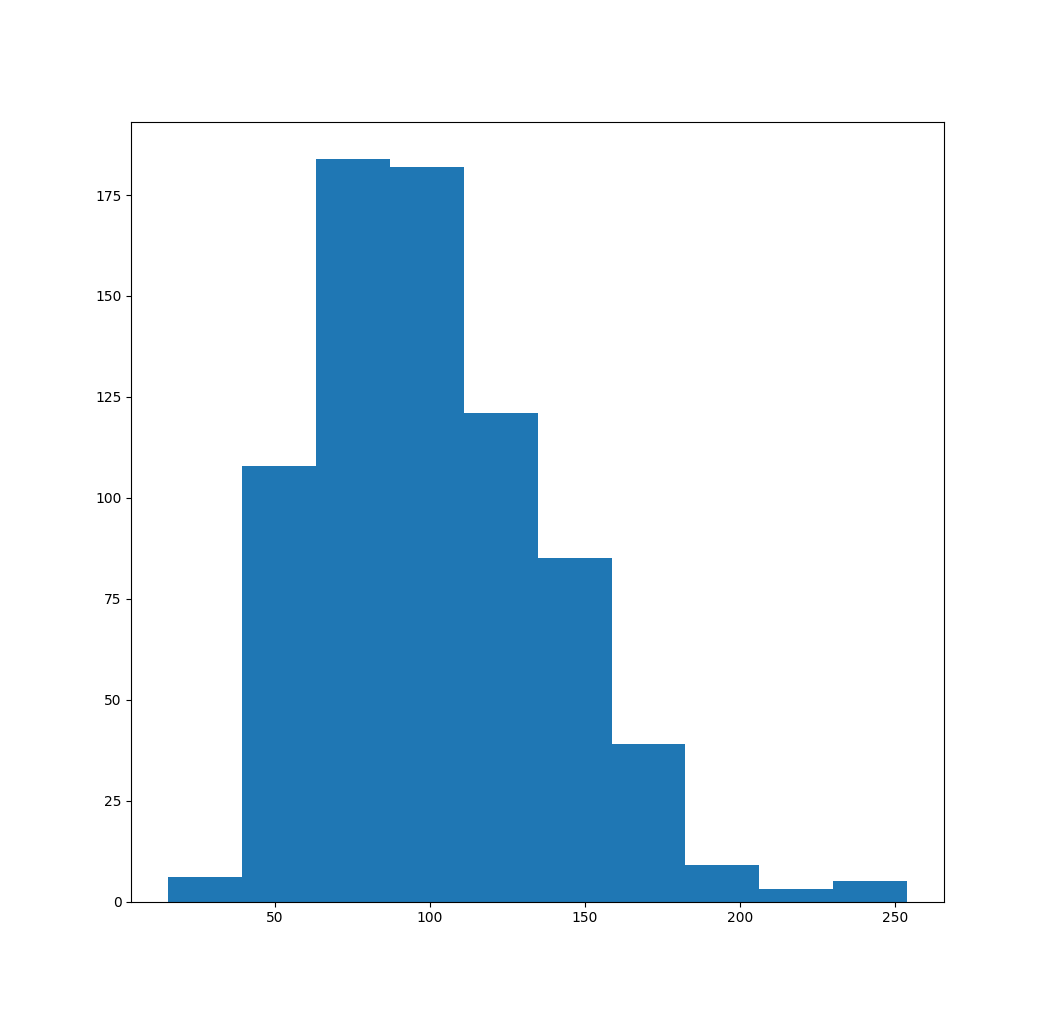
\includegraphics[width=6cm]{Figure_1.png}
\end{figure}
\end{frame}

\begin{frame}
\frametitle{Hipotesis 1}
\begin{figure}[t]
  \caption{Data estandarizada y sin outliers}
  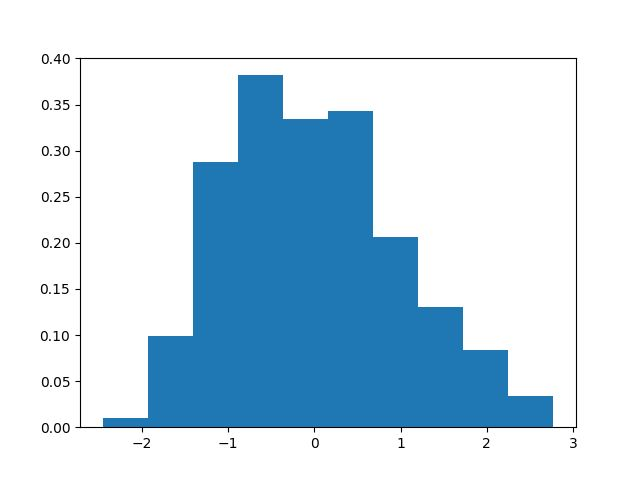
\includegraphics[width=6cm]{data_sin_outliers.jpeg}
\end{figure}
  \textbf{Puede parecer una distribucion Normal}

\end{frame}

\begin{frame}
\frametitle{Hipotesis 1}
\begin{figure}[t]
  \caption{Grafica Q-Q}
  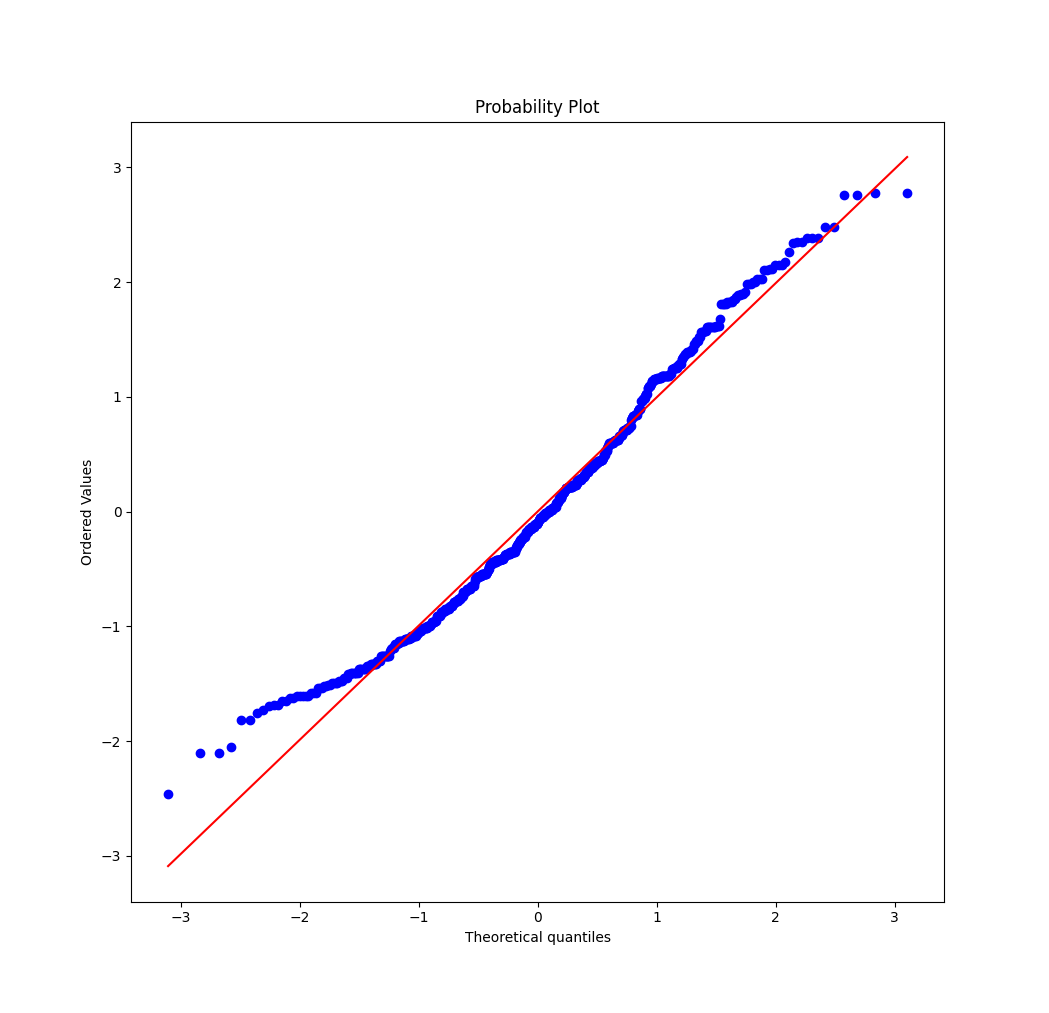
\includegraphics[width=6cm]{grafiaq-q.png}
\end{figure}
\end{frame}


\begin{frame}
\frametitle{Resultados hipotesis 1}
  Ever no te olvides del floro
\end{frame}

\begin{frame}
\frametitle{Hipotesis 2}
\begin{figure}[h]
  \caption{Distribución de ingresos de ingenieros de
  software en la India}
  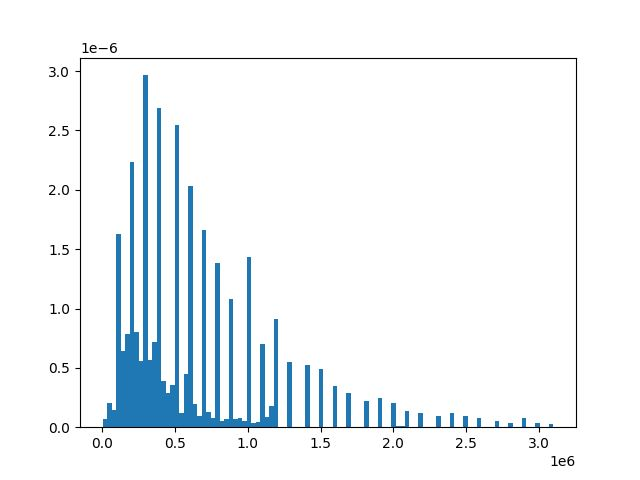
\includegraphics[width=8cm]{distribucion_ingresos_sw.jpeg}
\end{figure}

  se puede notar como existen \textit{2 grupos en la poblacion}
\end{frame}


\begin{frame}
\frametitle{Hipotesis 2}
\begin{figure}[h]
  \caption{Distribución de ingresos de ingenieros de
  software en la India}
  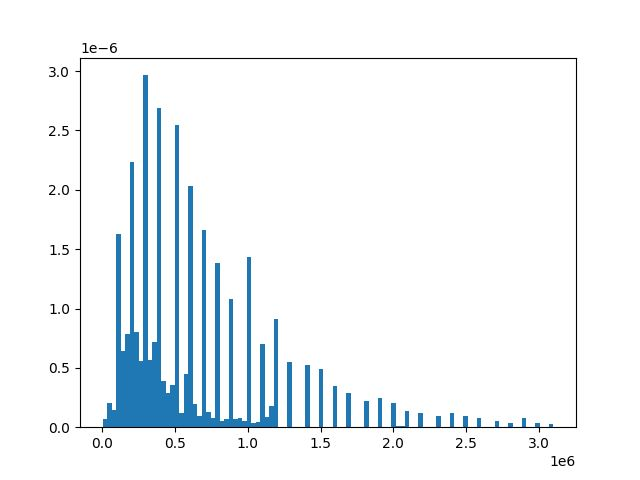
\includegraphics[width=8cm]{distribucion_ingresos_sw.jpeg}
\end{figure}

  se puede notar como existen \textit{2 grupos en la poblacion}
\end{frame}
\section{Conclusiones}

%---------------------------------------------------------
\begin{frame}
\frametitle{Conclusiones}

In this slide, some important text will be
\alert{highlighted} because it's important.
Please, don't abuse it.

\begin{block}{Remark}
Sample text
\end{block}

\begin{alertblock}{Important theorem}
Sample text in red box
\end{alertblock}

\begin{examples}
Sample text in green box. The title of the block is ``Examples".
\end{examples}
\end{frame}
%---------------------------------------------------------


%---------------------------------------------------------
%Two columns
\begin{frame}
\frametitle{Two-column slide}

\begin{columns}

\column{0.5\textwidth}
This is a text in first column.
$$E=mc^2$$
\begin{itemize}
\item First item
\item Second item
\end{itemize}

\column{0.5\textwidth}
This text will be in the second column
and on a second tought this is a nice looking
layout in some cases.
\end{columns}
\end{frame}
%---------------------------------------------------------

\end{document}
